\clearpage
\section{Hardware}\label{sec:Hardware}
In diesem Kapitel wird die Hardware vom \textit{Gateway Interface System}, dem \textit{Universal Peripheral Node}, dem \textit{Energy Harvesting System} und dem \textit{Power Storage System} beschrieben. 


\subsection{Bluetooth Mesh Node (BMN)}\label{subsec:BMN}
Im Bluetooth Mesh Protokoll gibt es zwei verschiedene  Geräte, ein \textit{"'unprovisioned device"'} und einen \textit{"'node"'}. Das \textit{"'unprovisioned device"'}  ist ein Teilnehmer, der für das Mesh Netzwerk unbekannt ist und deshalb keine Rechte besitzt. Wird dieses Gerät nun in das Netzwerk aufgenommen, so wird das \textit{"'unprovisioned device"'}  zu einem \textit{"'node"'}. Dieses vorgehen nennt sich \textit{"'provisioning"'}.\cite{afaneh_ultimate_2018} Die Hardware für den \textit{"'node"'} besteht bei allen Geräten aus dem gleichen SoC. Der nRF52840 von Nordic Semiconductor eignet sich aus folgenden Gründen perfekt für diese Anwendung. Die \textit{"'nodes"'} dürfen, um eine lange Laufzeit zu garantieren, sehr wenig elektrische Leistung beziehen. Der nRF52840 benötigt im Ruhemodus nur wenige $[\mu A]$. Ein weiterer Grund ist die sehr gute Dokumentation der Software von Nordic Semiconductor. Die gesamte Software ist im Infocenter erhältlich und frei zugänglich. Weitere Vorteile befinden sich in der Tabelle \ref{tbl:Vorteilte_nRF52}:\cite{nordic_semiconductor_nrf52840_2019} \\

\begin{table}[h]
	\begin{tabular}{ll}
		\multicolumn{2}{l}{{\ul \textbf{Vorteile des nRF52840}}}       \\
		Bluetooth 5                          											   & -95 dBm Sensivität      \\
		Multiprotokoll (Thread, Zigbee, usw) 						   & +8 dBm Ausgangsleistung \\
		Geringer Stromverbrauch  (wenige $[\mu A]$)      	& USB 2.0                 \\
		12bit ADC                            												& NFC                     \\
		1 MB flash und 256kB RAM Speicher    						& ARM M4F Cortex         
	\end{tabular}
	\caption{Vorteile des nRF52840}
	\label{tbl:Vorteilte_nRF52}
\end{table}


\begin{figure}[h]
	\centering
	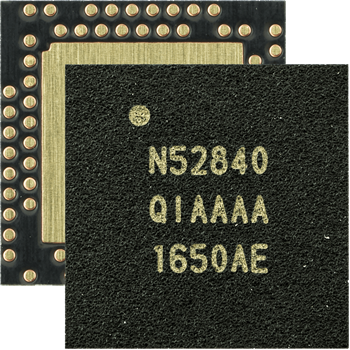
\includegraphics[scale=0.5,angle=0]{nRF52840.png}
	\caption{nRF52840 SoC \cite{nordic_semiconductor_nrf52840-qiaa.png_2019}}
	\label{img:nRF52840}
\end{figure} 

\subsection{Gateway Interface System (GIS)}\label{subsec:Gateway}
Der Bluetooth-Mesh-Gateway soll die Plattform gegenüber Fremdsystemen öffnen und damit die Schnittstelle zu IOT (Internet of Things) bilden. Damit die Plattform einfach zu betreiben ist, wird beim Gateway in erster Linie auf den Einplatinen-Computer Raspberry-Pi 4 (siehe Abschnitt \ref{img:raspberryPi4}) gesetzt. Andere Einplatinen-Computer wären ebenfalls denkbar wobei die Raspberry-Pi-Plattform bereits sehr weit verbreitet ist und somit oft bereits verfügbar ist.

Der Raspberry-Pi 4 besitzt nebst Ethernet und WLAN Schnittstellen sowie USB 3 Ports auch von Grund auf mit einem Bluetooth 5 Modul ausgestattet. So könnte er direkt ins Bluetooth-Mesh-Netzwerk integriert werden. Um jedoch die volle Integration zu erreichen, wird in erster Linie der oben erwähnte nRF52840 (siehe Abschnitt \ref{subsec:BMN}) in Form eines Dongle-Development-Boards \ref{img:nRF52840USBDongle} eingesetzt. Via serieller Schnittstelle wird dieser mit dem Raspberry-Pi 4 verbunden.


\begin{figure}[h]
	\centering
	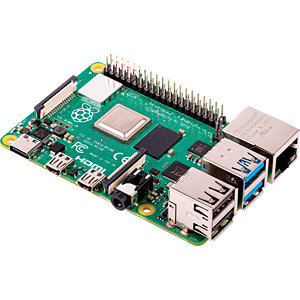
\includegraphics[scale=0.7,angle=0]{RASP_PI_4_B.jpg}
	\caption{Raspberry-Pi 4 \cite{reichelt_elektronik_gmbh_&_co_kg_rasp_nodate}}
	\label{img:raspberryPi4}
\end{figure} 

\begin{figure}[h]
	\centering
	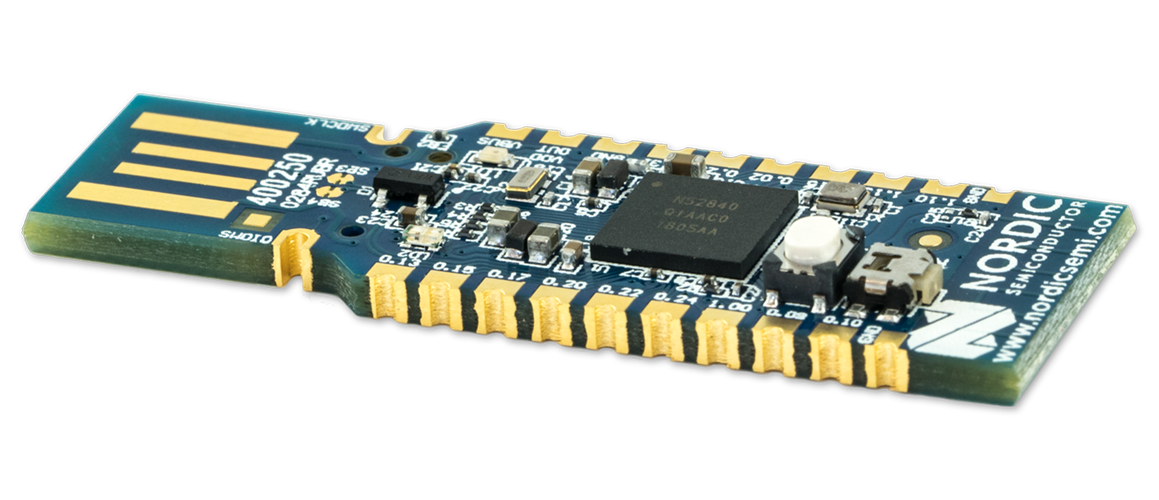
\includegraphics[scale=0.2,angle=0]{nRF52840_Dongle.png}
	\caption{nRF52840 USB Dongle \cite{nordic_semiconductor_nrf52840-dongle-promo.png_2019}}
	\label{img:nRF52840USBDongle}
\end{figure} 


\todo [inline] {Mobiltelefon soll den Gateway ersetzen. Ist als Wunschziel definiert.}

\subsection{Energy Harvesting System (EHS)}\label{subsec:EHS}

Das \textit{EHS} beinhaltet unterschiedlichen Methoden um Energie aus der Umgebung aufzufangen. Diese sind in der folgenden Tabelle mit den wichtigsten Kenndaten aufgefasst. 

\begin{figure}[h]
	\centering
	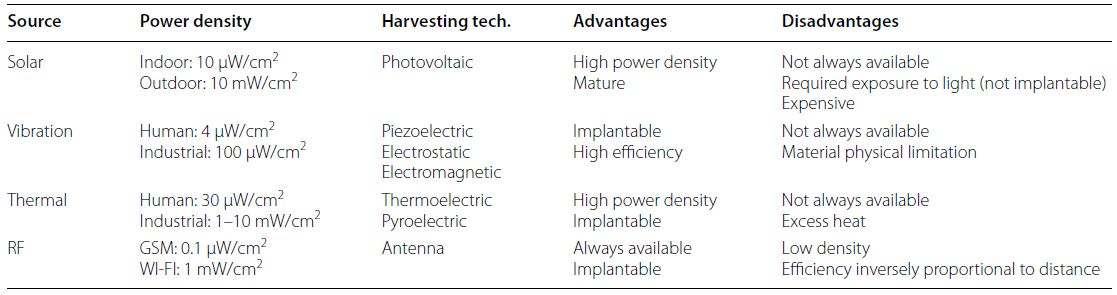
\includegraphics[scale=0.50,angle=0]{Tabelle_Energyharvesting_Sources.jpg}
	\caption{Tabelle Umgebungsenergie \cite{tran_rf_2017}}
	\label{img:Tabelle_Energyharvesting_Sources}
\end{figure} 

Durch Berechnungen, Simulationen und Testaufbauten soll gezeigt werden, welche Methode sich als genügend ertragreich für unser System erweist. Mithilfe der Ergebnisse soll es möglich sein, die optimale Konfiguration situationsbedingt zu wählen. 

\todo [inline]{Energiebudget (Wie viel wird benötigt?) muss im Projekt erstellt werden. Nur so kann EHS richtig ausgelegt werden.}

\subsection{Power Storage System (PSS)}\label{subsec:PSS}

Das \textit{PSS} ist für die Energiespeicherung zuständig. Untersucht wird die Speicherung der gewonnen Energie aus dem \textit{EHS} mithilfe Sekundärer Zellen (Akkus) oder mit \textit{Supercaps}. Zusätzlich soll die Versorgung aus primären Zellen untersucht werden. Mithilfe der Ergebnisse soll es möglich sein, die optimale Konfiguration situationsbedingt zu wählen.   
 

\todo [inline]{Abschaltung des Nodes um Tiefentladung des Speichers zu vermeiden --> evtl. BMS}